
\section{CRATE}
\label{sec:proposal}

\CRATE (stands for CollaboRATive Editor) is a distributed and decentralized
collaborative editor running directly inside web browsers.
Figure~\ref{fig:architecture} depicts \CRATE's architecture with four layers:
\begin{inparaenum}[(i)]
\item communication: includes the editing session membership mechanism and the
  information dissemination protocols.
\item causality: includes the causality tracking structure that guarantees a
  delivery order of operations reflecting a form of causality.
\item sequence structure: includes the structure that guarantees a global
  total order among elements of the sequence.
\item graphical user interface: includes the editor as a graphical entity that
  users can interact with inside web browsers.
\end{inparaenum}
The left part of the figure depicts the common process chain: when the user
performs an operation on the document, the operation is applied to the shared
sequence which creates an \LSEQ identifier. Then it decorates the result of the
operation with causality tracking metadata. Finally, \CRATE broadcasts it using
the neighborhood provided by the \SPRAY random peer sampling protocol.
Conversely, when \CRATE receives a broadcast message, it checks if the operation
is causally ready to be delivered. Once the condition is verified, it applies
the operation to the shared sequence which notifies the graphical user interface
of the changes.  The right part of the figure corresponds to the catch up
strategy where a peer may have missed operations due to dropped messages, or
simply because the peer worked on offline mode for a while. Therefore, it
regularly asks to its neighborhood the missing operations using the differences
of version vectors.

The rest of this section reviews each layer and details the component inside
them.

\begin{figure}
  \centering
  \begin{tikzpicture}[scale=1.1]

\newcommand\X{25pt}
\newcommand\Y{20pt}

\newcommand\LIGHTGRAY{gray!20}

\small
%% communication
\draw[rounded corners=2mm, fill=white](0pt, 0pt)+(-4*\X,-\Y)rectangle+(4*\X,\Y);
\draw(4*\X, \Y)node[anchor=north east]{\textbf{communication}};

\draw[fill=white](-2*\X, -0.25*\Y)
node{broadcast}+(-0.75*\X,-0.5*\Y)rectangle+(0.75*\X,0.5*\Y);
\draw[fill=white, thick]( 0*\X, 0.25*\Y)
node{\SPRAY}+(-0.75*\X,-0.5*\Y)rectangle+(0.75*\X,0.5*\Y);
\draw[fill=white]( 2*\X, -0.25*\Y)
node{unicast}+(-0.75*\X,-0.5*\Y)rectangle+(0.75*\X,0.5*\Y);

\draw[<-](-0.75*\X, 0.25*\Y)--(-1.25*\X, -0.25*\Y);
\draw[<-](0.75*\X, 0.25*\Y)--(1.25*\X, -0.25*\Y);

%% causality
\draw[rounded corners=2mm, fill=\LIGHTGRAY](0pt, -2*\Y)+(-4*\X,-\Y)rectangle+(4*\X,\Y);
\draw(4*\X, -\Y)node[anchor=north east]{\textbf{causality}};

\draw[fill=\LIGHTGRAY](-2*\X, -2*\Y)
node[align=center]{version vector\\with\\exceptions}
+(-1.0*\X,-0.6*\Y)rectangle+(1.0*\X,0.6*\Y);

\draw[<->, thick](-2*\X, -0.75*\Y)--(-2*\X, -1.4*\Y);
\draw[<->]( 2*\X, -0.75*\Y)--( 1*\X, -2.5*\Y);

%% sequence structure
\draw[rounded corners=2mm, fill=white](0pt, -4*\Y)+(-4*\X,-\Y)rectangle+(4*\X,\Y);
\draw(4*\X, -3*\Y)node[anchor=north east, align=right]
{\textbf{sequence}\\\textbf{structure}};

\draw[fill=white, shading=axis,top color=\LIGHTGRAY, bottom color=white, shading angle=0](1*\X, -3*\Y)
node{anti-entropy}+(-0.95*\X,-0.5*\Y) rectangle +(0.95 *\X, 0.5*\Y);
\draw[fill=white, thick](-2*\X, -4*\Y)
node{\LSEQ}+(-0.75*\X,-0.5*\Y) rectangle +(0.75 *\X, 0.5*\Y);

\draw[->] (0.05*\X, -2.75*\Y)--(-1*\X,-2*\Y);
\draw[->] (0.05*\X, -3.25*\Y)--(-1.25*\X,-4*\Y);
\draw[<->, thick] (-2*\X, -3.5*\Y)--(-2*\X, -2.6*\Y);

%% gui
\draw[rounded corners=2mm, fill=\LIGHTGRAY](0pt, -6*\Y)+(-4*\X,-\Y)rectangle+(4*\X,\Y);
\draw(4*\X, -5*\Y)node[anchor=north east, align=right]
{\textbf{graphical}\\\textbf{user}\\\textbf{interface}};
\draw[fill=\LIGHTGRAY](0pt,-6*\Y)
node{web editor}+(-0.85*\X,-0.5*\Y) rectangle +(0.85 *\X, 0.5*\Y);

%%\draw[<->] (-2*\X, -4.5*\Y) -- (0*\X, -5.5*\Y);
\draw[<->, thick] (-2*\X, -4.5*\Y) -- (-0.85*\X, -6*\Y);
\end{tikzpicture}
  \caption{\label{fig:architecture}The four layers of \CRATE's architecture}
\end{figure}

\subsection{Communication}
To collaboratively edit a document, users must establish a form of communication
between them. It firstly requires to build a network of communication
channels. It secondly requires to use it to disseminate the changes performed on
the shared document to all participants.  \CRATE uses
\SPRAY~\cite{nedelec2015spray} as membership protocol and relies on its
properties to efficiently disseminate the messages.

\begin{asparadesc}
\item [The membership protocol,] called \SPRAY, is a random peer sampling
  protocol~\cite{jelasity2007gossip} the primary target of which is WebRTC, a
  recent technology that allows peer-to-peer communication between web browsers.
  As such, the range of users includes small devices (e.g. smartphones, tablets,
  etc.) and establishing a connection requires a three-way handshake. These
  constraints invite to maintain a small number of connections.

  Using \SPRAY, each member owns a set of neighbors which dynamically grows and
  shrinks to reflect the network size. Without any global knowledge,
  \begin{inparaenum}[(i)]
  \item it provides each member with a neighborhood of logarithmic size compared
    to the global network size;
  \item it quickly converges to a topology exposing similarities with random
    graphs~\cite{erdos1959random}. Among others,
    \begin{inparaenum}[(a)]
    \item it balances the load among members by repeatedly averaging over time the
      size of neighborhoods pairwise;
    \item it becomes robust to random crashes or unexpected departures of
      members;
    \item the shortest average distance to reach all peers stays small.
    \end{inparaenum}
  \end{inparaenum}
  
  \SPRAY divides the life-cycle of a member into three phases: the joining, the
  exchanges, and the leaving. They respectively aim to increase, retain, and
  decrease the number of connections to follow a logarithmic progression.

\item [The information dissemination protocol]\cite{birman1999bimodal} aims to
  propagate the changes performed by the user on their shared document. Any
  operation must reach all members (broadcast) to guarantee eventual
  consistency. The dissemination relies on the neighborhood provided by
  \SPRAY. When a user performs an operation, \CRATE prepares a message including
  the result of the operation and sends it to the whole network using its
  neighborhood. Neighbors receiving such message forward it to their own
  neighbors. Hence, messages reach all participants transitively. To guarantee
  termination and limit the flooding, each member forwards each message to their
  neigbhors only once by using a version vector with exceptions
  (cf. Section~\ref{subsec:causality}).

  The information dissemination protocol impacts the communication complexity at
  each peer:
  \begin{equation}
    \mathcal{O}(m.\ln |\mathcal{R}| )
  \end{equation}
  where $m$ is the message size determined by the layers below, and
  $|\mathcal{R}|$ is the number of replicas in the network including both
  writers and readers of the shared sequence.
\end{asparadesc}

\subsection{Causality tracking}
\label{subsec:causality}

The causality tracking layer guarantees that operations are not delivered more
than once, and that operations depending on another operation is delivered after
the latter. \CRATE uses a version vector with
exceptions~\cite{malkhi2007concise} which stores for each site
\begin{inparaenum}[(i)]
\item an integer denoting the maximum counter of operations originated from this
  site and
\item a list of integers denoting the exceptions, i.e., the counter of
  operations known as not received yet.
\end{inparaenum}

Each operations is uniquely identified by its unique site identifier and a
monotonically growing counter. On operation reception, \CRATE discards the
operation if it has already been received before. Otherwise, it modifies the
version vector entry either by updating the maximum counter or removing an entry
in the exceptions.

\begin{figure}
  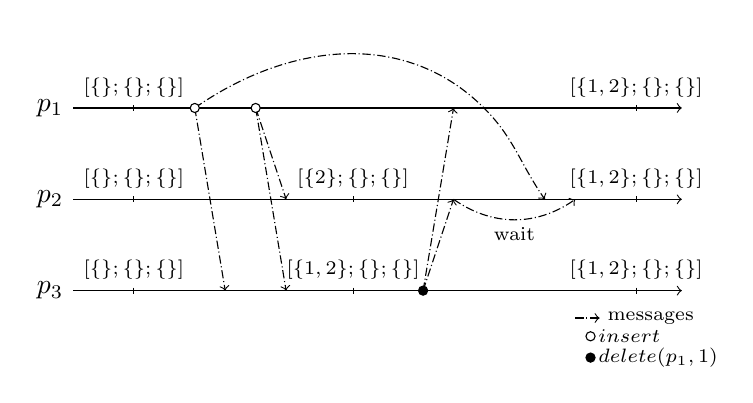
\begin{tikzpicture}[scale=1.1]
  
  \draw (-10pt,0pt) node[anchor=east]{$p_1$};
  \draw (-10pt,-30pt) node[anchor=east]{$p_2$};
  \draw (-10pt,-60pt) node[anchor=east]{$p_3$};

  \draw[->] (-10pt,0pt) -- (190pt,0pt);
  \draw[->] (-10pt,-30pt) -- (190pt,-30pt);
  \draw[->] (-10pt,-60pt) -- (190pt,-60pt);

  \scriptsize
  \draw (10pt,1pt) node[anchor=south]{[$\{\};\{\};\{\}]$} --
  (10pt,-1pt);
  \draw (10pt,-29pt) node[anchor=south]{[$\{\};\{\};\{\}]$} --
  (10pt,-31pt);
  \draw (10pt,-59pt) node[anchor=south]{[$\{\};\{\};\{\}]$} --
  (10pt,-61pt);

  \draw[->,densely dashdotted] (30pt,0pt) -- (40pt,-60pt);
  \draw[->,densely dashdotted] (50pt,0pt) -- (60pt,-30pt);
  \draw[->,densely dashdotted] (50pt,0pt) -- (60pt,-60pt);


  \draw (82pt,-29pt) node[anchor=south]{[$\{2\};\{\};\{\}]$} --
  (82pt,-31pt);
  \draw (82pt,-59pt) node[anchor=south]{[$\{1,2\};\{\};\{\}]$} --
  (82pt,-61pt);

  \draw [->,densely dashdotted] (30pt,0pt) to[out=35,in=135] (125pt,0pt)
  to[out=-45,in=125] (145pt,-30pt);

  \draw[fill=white] (30pt,0pt) circle (1.5pt);
  \draw[fill=white] (50pt,0pt) circle (1.5pt);

  \draw[->,densely dashdotted] (105pt,-60pt)--(115pt,-30pt);
  \draw[->,densely dashdotted] (105pt,-60pt)--(115pt,0pt);

  \draw[fill=black] (105pt,-60pt) circle (1.5pt);
  
  \draw[->,densely dashdotted]
  (115pt,-30pt)to[out=-35,in=-145]node[anchor=north]{wait}(155pt,-30pt);


  \draw (175pt,1pt) node[anchor=south]{$[\{1,2\};\{\};\{\}]$}-- (175pt,-1pt);
  \draw (175pt,-29pt) node[anchor=south]{$[\{1,2\};\{\};\{\}]$}--(175pt,-31pt);
  \draw (175pt,-59pt) node[anchor=south]{$[\{1,2\};\{\};\{\}]$}--(175pt,-61pt);
  
  \draw[->,densely dashdotted] (155pt,-69pt) -- (163pt,-69pt)
  node[anchor=west]{messages};
  \draw[fill=white] (160pt,-75pt)node[anchor=west]{$insert$}circle (1.5pt);
  \draw[fill=black] (160pt,-82pt)
  node[anchor=west]{$delete(p_1,1)$} circle (1.5pt);

\end{tikzpicture}

  \caption{\label{fig:timeline}Causality tracking example.}
\end{figure}

Figure~\ref{fig:timeline} depicts a scenario where 3 peers are involved. Thus,
all peers have a vector of three entries. Peer $p_1$ inserts two elements in the
sequence and broadcasts the operations. Peer $p_3$ immediately receives both
operations and increments the entry in its version vector accordingly.  In the
meantime, Peer $p_2$ only receives the second operation which leads to an update
of the maximum counter and an exception concerning the first operation of Peer
$p_1$. Then, Peer $p_3$ removes the first element inserted by $p_1$ and
broadcast it. While $p_1$ delivers the removal immediately, Peer $p_2$ has to
wait since the targeted operation belongs to the exceptions. Once it receives
the first operation of $p_1$, the exception disappears and the delete operation
is performed.

The local space complexity of such data structure depends of the number of
writers $|\mathcal{W}|$, i.e., the users that modified the document at least
once:
\begin{equation}
  \mathcal{O}(|\mathcal{W}|)
\end{equation}
The communication complexity is not impacted from this data
structure. Therefore, its becomes:
\begin{equation}
  \mathcal{O}(o.\ln |\mathcal{R}|)
\end{equation}
where $o$ is the operation size determined by the shared sequence structure,
and the rest is determined by the communication layer.

The anti-entropy periodically checks if the local replica diverges from another
neighbor's one at random. It aims to retrieve missing operations that could have
been lost during the transmissions. \TODO{example}. There is no additional cost
on local memory. However, the communication cost is prohibitively high which
encourages to perform this reconciliation protocol with great care:
\begin{equation}
  \mathcal{O}(|\mathcal{W}|+|\mathcal{W}|+x.o)
\end{equation}
where the first $|\mathcal{W}|$ designates the initiating message, and
$|\mathcal{W}|+x.o$ the response to this message where $x.o$ are the missing
operations.

\subsection{Shared sequence}
The shared sequence layer uses a conflict-free replicated data type for
sequences~\cite{shapiro2011comprehensive, shapiro2011conflict}. It is an
abstract data type for sequences that provides two commutative operations:
insert and delete. As such, the delivery order of operations does not matter as
long as the deletion of an element follows its insertion. This property makes
these shared sequences tolerant to concurrency. However, their complexity lies
in their space consumption. Indeed, each insert operation allocates a unique and
immutable identifier to the element. A global total order among the identifiers
guarantees that replicas eventually converge to an identical states.

\CRATE uses \LSEQ, a polyLogarithmic identifier allocator for SEQuences. Its
underlying structure is an exponential tree which, when linearized using its
global total order, results in the sequence of elements representing the
document. \LSEQ comprises two parts:
\begin{inparaenum}[(i)]
\item the function $allocPath$ which chooses the path in the tree for the
  newly allocated identifier.
\item the function $allocDis$ which decorates the path in order to ensure its
  uniqueness even in presence of concurrent insertions.
\end{inparaenum}

The function $allocPath$ chooses the path associated with each element in order
to encode its relative position with regard to its adjacent elements in the
sequence. For the sake of performance, the aim of $allocPath$ is to keep the
underlying tree with a small depth. Three components compose $allocPath$. Each
of these components fails to provide an efficient allocation
function. Nevertheless, their composition allows to get the best of each by
canceling their respective deficiency.
\begin{asparadesc}
\item [An exponential tree]~\cite{andersson1996faster,andersson2007dynamic}
  represents the shared document. The path is a sequence of numbers chosen among
  a subset of numbers the size of which is doubled at each concatenation. For
  instance, if a path $p_1$ of size 1 is chosen among [$\mathbb{N}_{<32}$], a
  path $p_2$ of size 2 is chosen among [$\mathbb{N}_{<32}.\mathbb{N}_{<64}$]
  etc. Let $r$ be the number of possible paths with one concatenation (i.e., the
  maximum arity of the root of the tree), a path $p_k$ of size $k$ is chosen
  among [$\mathbb{N}_{<r}.\mathbb{N}_{<2r}\ldots\mathbb{N}_{<2^{k-1}r}$].  Due
  to the growth of the subsets, such representation of the paths requires one
  additional bit to encode each concatenation. With the same examples, it
  implies that $p_1$ is encoded using $log_2(32)=5$ bits, $p_2$ is encoded using
  $5+6=11$ bits,~\ldots Thus, a path is encoded by:
  \begin{equation}
    \sum\limits_{i=1}^{k}(\log_2(r)+i) =
    k\log_2(r) + {k(k+1)\over{2}} = \mathcal{O}(k^2) \,\, bits
  \end{equation}
  When an exponential tree of depth $k$ is balanced (i.e., all its branches
  are filled) it holds uptil:
  \begin{equation} \sum\limits_{i=0}^{k-1} {2^{(i^2-i)/2}} \,\, elements
  \end{equation}
  When an exponential tree of depth $k$ has one branch filled per level, it
  holds uptil:
  \begin{equation} 2^{k+1}-1 \,\, elements\end{equation} 
  In the worst case, the tree contains one element per level.
  
  An alphabetical order maintains a dense total order among elements in the
  tree. It primary uses the path of elements alongside globally unique markers
  called disambiguators. The latter's objective is twofold:
  \begin{inparaenum}[(i)]
  \item to order concurrent operations that happen to have an identical path and
  \item to allow the allocation of new identifiers in-between them.
  \end{inparaenum}
  For instance, let [3] be the path of Element Q inserted by User $u_x$, and let
  [4] the path of Element T inserted by User $u_y$. When a user $u_1$ inserts W
  between those elements, the depth of the tree must grow to welcome the new
  element. Assuming that depth 1 has a maximum arity of 8, the identifier is
  allocated in the range from [3.0] to [3.15].  In this example, the resulting
  path is [3.6]. In the meantime, another user $u_2$ inserts R between Q and T
  which happens to result in the path [3.6] too. To ensure a total order,
  disambiguators are associated with each path composed of a monotonically
  growing counter and a globally unique site identifier. Here, the identifier of
  Element W is composed of the path [3.6] and disambiguator
  [$\langle u_x,\,1\rangle$, $\langle u_1,\,1$] and the Element R is composed of
  the path [3.6] and disambiguator [$\langle u_x,\,1\rangle$,
  $\langle u_2,\,1\rangle$].  The comparison starts to examine the first
  concatenations which are equal.  Then, the comparison concerns the path of the
  second level of the tree which are equals too. Hence, it examines the
  disambiguators to determine that W is located before R because $u_x < u_y$ in
  this case. The resulting sequence is QWRT.
  
\item [Two sub-allocation functions] designed for monotonic editing, i.e.,
  inserting repeatedly at an adjacent position of the previously inserted
  element. These are application dependent. While one is well-suited to
  end-editing (left-to-right), the other is well-suited for front-editing
  (right-to-left). To achieve this, they respectively allocate paths close of
  the leftmost path, and rightmost path in order to preserve space for the
  future insertions. Hence, the left-to-right allocation function leaves
  available paths at the right of the tree, while the right-to-left function
  aims the opposite. For instance, a user writes QWERTY starting from the Q to
  the Y. Using the left-to-right allocation function leads to identifiers like
  [2], [4], [7], [7.2], [7.5], [7.9]. Small space is left in-between paths to
  handle mistakes, e.g., a user misses some characters while typing.  Since
  accurately predicting the editing behavior of users is \TODO{impossible},
  \LSEQ uses these two antagonist strategies to adapt to any editing behaviors
  assuming that edition is mostly about compositions of sequences of monotonic
  insertions.
  
\item [A hash function] chooses among the two sub-allocation functions. The
  choice is made randomly using a hash function following a uniform
  distribution. Such function does not favor any editing behavior while
  remaining efficient. This provides the independence of the allocation function
  from any editing strategy. Furthermore, as shown
  in~\cite{nedelec2013concurrency}, using antagonist sub-allocation functions
  forces all peers to make identical choices. To reach that goal, they all use a
  similar hash function initialized with a common seed and shared within the
  document. When a user inserts a new element in the sequence, \LSEQ firstly
  processes the depth of the new path, and secondly defers the allocation to the
  function designated by the hash of the depth.
\end{asparadesc}

% \begin{algorithm}[h]
%   
\begin{algorithmic}[1]

\small
\algrenewcommand{\algorithmiccomment}[1]{\hskip2em$\rhd$ #1}
\newcommand*{\comment}[1]{$\rhd$ #1}

  \State \textbf{let} $boundary \leftarrow 10$; \hfill \comment{Any constant}
  \label{line:boundary}
  \State \textbf{let} $h:\mathbb{N} \rightarrow (\mathcal{P}\times
  \mathcal{P}\rightarrow \mathcal{P})$; \hfill \comment{get sub-allocation
    function}
  \Statex
    \Function{allocPath}{$p,\, q \in \mathcal{P}$}
    $\rightarrow \mathcal{P}$
    \State \textbf{let} $\langle depth,\,\_ \rangle 
    \leftarrow \textsc{getDepthInterval}(p,\,q)$;
    \State \textbf{return} $h(depth)(p,\,q)$; 
    \hfill \comment{Delegates the call}
    \EndFunction
    \Statex
    \Function{left-to-right}{$p,\,q \in \mathcal{P}$}\label{line:lefttoright}
    $\rightarrow \mathcal{P}$
    \Statex \comment{\#1 Get the depth of the new path}
    \State \textbf{let} 
    $\langle depth,\,interval \rangle \leftarrow \textsc{getDepthInterval}(p,\,q);$
    \Statex \comment{\#2 Maximal space between two identifiers}
    \State \textbf{let} $step \leftarrow min(boundary,\,interval)$;
    \Statex \comment{\#3 Create the new path}\label{line:plus}
    \State \textbf{return} $\textsc{subPath}(p,\,depth) + rand(0,\,step)$;
    \EndFunction
    \Statex
    \Function{right-to-left}{$p,\,q \in \mathcal{P}$}\label{line:righttoleft}
    $\rightarrow \mathcal{P}$
    \State \textbf{let}
    $\langle depth,\, interval\rangle \leftarrow \textsc{getDepthInterval}(p,\,q);$
    \hfill \comment{\#1}
    \State \textbf{let} $step \leftarrow min(boundary,\,interval)$;
    \hfill \comment{\#2}
    \State \textbf{return} $\textsc{subPath}(q,\,depth) - rand(0,\,step)$;
    \hfill \comment{\#3}\label{line:minus}
    \EndFunction
    \Statex
    \Function{getDepthInterval}{$p,\,q \in \mathcal{P}$} $\rightarrow \mathbb{N} \times \mathbb{N}$
    \Statex   \comment{Which level has enough space for 1 path} 
      \State \textbf{let} $d \leftarrow 0$; \hfill \comment{depth}
      \State \textbf{let} $interval \leftarrow 0$;
      \While{$(interval < 2)$}
        \State $d \leftarrow d + 1$;
        \State $interval \leftarrow \textsc{subPath}(q,\,d) - \textsc{subPath}(p,\,d)$;
      \EndWhile
      \State \textbf{return} $\langle d,\, interval\rangle$;
    \EndFunction

  \end{algorithmic}


%   \caption{The $allocPath$ function of \LSEQ}
%   \label{algo:allocpathalgo}
% \end{algorithm}
  

% \begin{algorithm}
%   \input{input/allocdesalgo.tex}
%   \caption{\label{algo:allocdis}The function $allocDis$ of \LSEQ}
% \end{algorithm}

% In text editing, most of the editing behaviors can be empirically summarized
% as a composition of two basic editing behaviors.
% \begin{inparaenum}[(i)]
% \item The random editing behavior where the author inserts new elements at
%   what appears random positions in the sequence. For instance, this behavior
%   mostly arises when syntactic corrections are performed, e.g., the author
%   writes $QWETY$ and realizes that the $R$ is missing. She adds the missing
%   character in a second time.
% \item The monotonic editing behavior where the author repeatedly inserts new
%   elements between the last inserted element and an adjacent element (after or
%   before exclusively). For instance, when an author writes $QWERTY$, she
%   generally starts from the first letter $Q$ to the last letter of the word
%   $Y$. On the opposite, insertions in a logfile are usually performed at the
%   beginning for practical reasons.
% \end{inparaenum}

% As a consequence, we focus on the space complexity analysis of \LSEQ to
% random and monotonic editing behaviors to which we add a worst-case complexity
% analysis.  The analysis does not include an average case since it requires to
% know the average distribution of the position of edits performed by a human
% collaborator which is obviously very complex.

\begin{table*}
  \centering
  
\begin{tabular}{@{}lccccccc@{}}
  \toprule
  \textsc{Editing behavior} & \multicolumn{2}{c}{\textsc{Space}} & \multicolumn{5}{c}{\textsc{Time}} \\ \cmidrule{4-8}
  & & & \multirow{2}{*}{\textsc{Lookup}} & \multicolumn{2}{c}{\textsc{Local}} & \multicolumn{2}{c}{\textsc{Remote}} \\ \cmidrule{2-3} \cmidrule{5-8}
  & \textsc{Identifier} & \textsc{Sequence} & & \textsc{ins} & \textsc{del} & \textsc{ins} & \textsc{del}  \\ \midrule
  Random editing & $\mathcal{O}(\log I)$ & $\mathcal{O}(I\log I)$ & $\mathcal{O}(2^{\sqrt{\log I}})$ & $\mathcal{O}(\sqrt{\log I})$ & $\mathcal{O}(1)$ & $\mathcal{O}(\log I + \sqrt{\log I})$ & $\mathcal{O}(\log I + \sqrt{\log I})$ \\
  Monotonic editing & $\mathcal{O}((\log I)^2)$ & $\mathcal{O}(I \log I)$ & $\mathcal{O}(I)$ & $\mathcal{O}(\log I)$ & $\mathcal{O}(1)$ & $\mathcal{O}((\log I)^2 +\log I)$ & $\mathcal{O}((\log I)^2 +\log I)$ \\
  Worst case & $\mathcal{O}(I^2)$ & $\mathcal{O}(I^2)$ & $\mathcal{O}(I)$ & $\mathcal{O}(I)$ & $\mathcal{O}(1)$ & $\mathcal{O}(I)$ & $\mathcal{O}(I)$\\ \bottomrule
\end{tabular}


%%  Id.size & $O(\sqrt{log\,n})$ & $O(log\,n)$ & $O(n)$ \\ \midrule
%%  Id.bit-length & \multicolumn{3}{c}{ $\sum\limits_{i=1}^{k}b+i =
%%                  kb + k(k+1)/2 = O(k^2)$} \\ \midrule
%%  Space complexity & $O(log\,n)$ & $O((log\,n)^2)$ & $O(n^2)$ \\ \bottomrule
  \caption{\label{table:lseqcomplexities}
    Upper-bound on space and time complexities of \LSEQ. Where $I$ is the number
    of insert operations performed.}
\end{table*}

\TODO{To summarizes, the space complexity analysis reveals that the allocation
function \LSEQ sacrifices on the worst-case space complexity to improve the
space complexity of the monotonic editing behaviors. Nevertheless, in text
editing, the worst-case happens with a very low probability compared the other
cases. Furthermore, it is worth noting that usually, the authors do not write a
document in a single round, starting from the beginning to go straight up to
the end (as the monotonic analysis could suggest). On the contrary, the authors
write sections, structure the documents, perform corrections, rewrite parts of
the document, reorganize, etc. This behavior (between random and monotonic
behavior) tends to even up the branches of the underlying tree of \LSEQ. In
the case of random editing, the space complexity is asymptotically optimal
$O(log\,n)$ while it is very interesting in a "normal setting" $O((log\,n)^2)$.}

\begin{figure*}
  \centering
  \subfloat {\input{input/lseqtreeexampleA.tex}}
  \hspace{10pt}
  \subfloat {\input{input/lseqtreeexampleB.tex}}
  \caption{\label{fig:lseqtreeexample}\LSEQ tree handling two monotonic
    editing behaviors.}
\end{figure*}


Figure~\ref{fig:lseqtreeexample} depicts the resulting trees after two
antagonist scenarios creating the sequence $QWERTY$
\begin{inparaenum}[(i)] 
\item the left-to-right editing sequence [($Q,\,0$), ($W,\,1$), \ldots] and
\item the right-to-left editing sequence [($Y,\,0$), ($T,\,0$), \ldots].
\end{inparaenum}
In both cases, the exponential tree of \LSEQ starts with an arity $32$ and
doubles it at each level. Also, it uses the $frontEditing$ and $endEditing$
sub-allocation functions at the first and the second level of the tree
respectively. Since the first level of the tree uses the function $endEditing$,
the scenario involving the left-to-right editing sequence results in a tree of
depth 1. On the other hand, contrarily to the allocation function presented in
Figure\ref{fig:allocpathexample}), the antagonist scenario does not increase
very much the depth of the tree. Indeed, the identifiers of \LSEQ quickly reach
a level of the tree where the sub-allocation function is designed to handle the
right-to-left editing behavior.


%%% Local Variables: 
%%% mode: latex
%%% TeX-master: "../paper"
%%% End: 

% LocalWords:  disambiguator neighbours
